\section{Anforderungen TourLive Server}
\label{sec:tourliveusecase}
\subsection{Live Stream}
Auf der Webseite werden Bilder von den Aufnahmegeräten zum aktuellen Zeitpunkt angezeigt. Auf den Bildern ist zu erkennen, wann dieses erstellt wurde. Das Bild kann zusätzlich vergrössert werden. Je nach Einstellung werden stehende Bilder (wie in Abbildung 1) oder fliessende Bilder (Videos) übertragen
\begin{figure}[H]
	\centering
	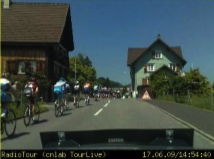
\includegraphics[height=60mm]{images/tourliveweb/tourliveaufnahme.png}
	\caption{Aufnahme aus dem Fahrzeug}
\end{figure}

\subsection{Streckenprofil}
Der Verlauf der Strecke wird in einem Streckenprofil dargestellt. Die Position der Aufnahmegeräte wird mit verschiedenen Farben aufgezeichnet, das Streckenprofil an sich ist statisch und beinhaltet zusätzliche Renn-Informationen wie z.B. Sprints oder Passhöhen. Die Zusatzinformationen und Profildaten werden von Bildern, GPS-Daten und/oder der Marschtabelle übernommen.
\begin{figure}[H]
	\centering
	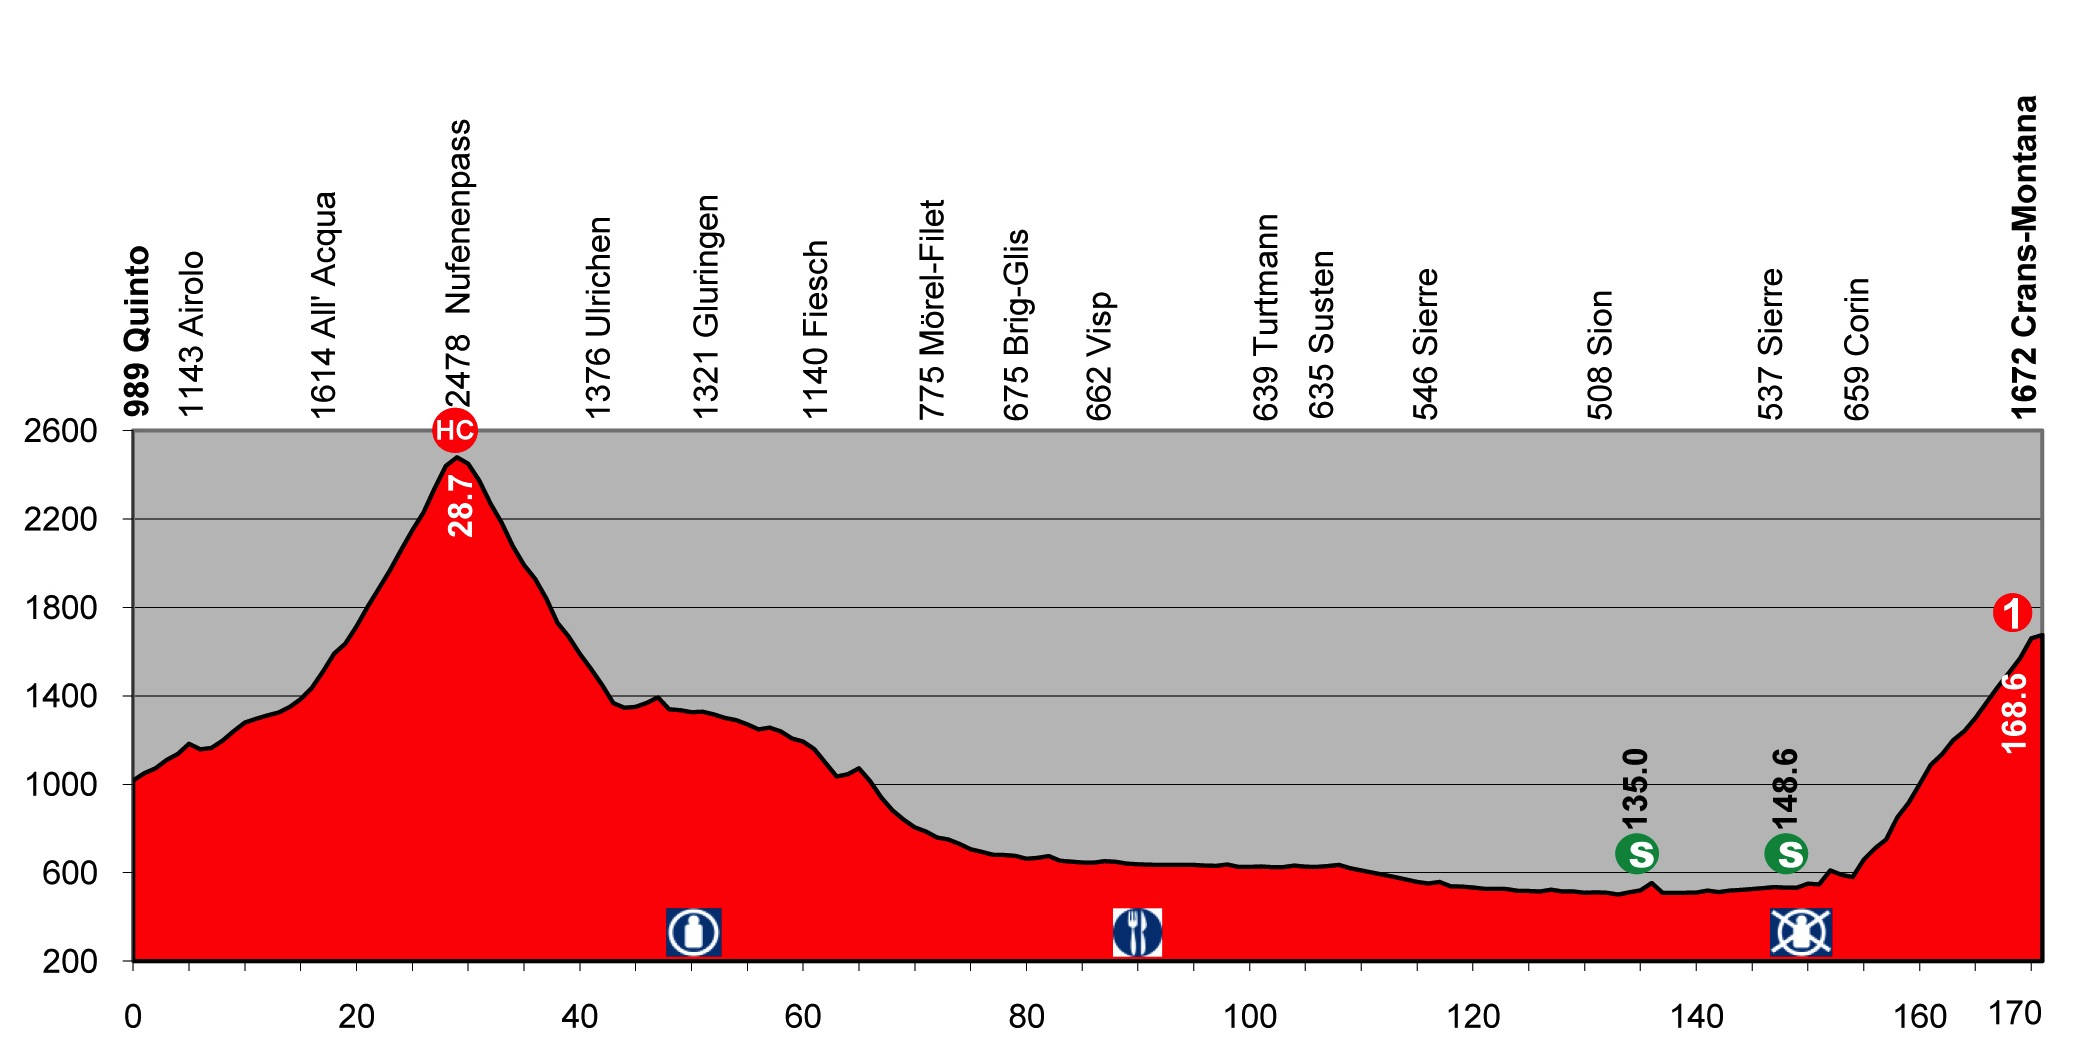
\includegraphics[width=130mm]{images/tourliveweb/streckenprofil.jpg}
	\caption{Streckenprofil aus der Tour de Suisse 2013\footnote{Bildquelle: \url{http://tourdesuisse.ch}, Aufgerufen am 08.05.2013}}
\end{figure}

\subsection{Abstände}
Jedes Aufnahmegerät zeichnet unter anderem die aktuelle Geschwindigkeit auf, diese wird wie in Abbildung 3 dargestellt. Der Server versucht zusätzlich die Distanz zwischen den Geräten zu berechnen und zeigt diese zusammen mit dem zeitlichen Rückstand an. Der TourSpeaker kann zusätzlich den Abstand in der Figur überschreiben, sofern diese Daten aktueller sind
\begin{figure}[H]
	\centering
	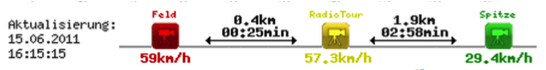
\includegraphics[width=130mm]{images/tourliveweb/abstaende.png}
	\caption{Abstände zwischen den Aufnahmesystemen}
\end{figure}

\subsection{Rennsituation}
Die gegenwärtige Rennsituation wird grafisch dargestellt, bei kleineren (Verfolger-) Gruppen werden die Fahrer namentlich aufgelistet, beim Feld wird nur die gesamte Anzahl Fahrer angezeigt. Der Vorsprung bzw. Rückstand ist bei allen Gruppen relativ zur Spitze angegeben. Zusätzlich wird der letzte Wert ebenfalls angegeben, um eine allfällige Tendenz feststellen zu können.
\begin{figure}[H]
	\centering
	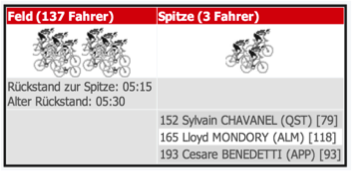
\includegraphics[width=80mm]{images/tourliveweb/rennsituation.png}
	\caption{Die aktuelle Rennsituation dargestellt}
\end{figure}
\subsection{Ranglisten}
Aus der aktuellen Rennsituation lässt sich eine virtuelle (Live) Rangliste bestimmen. Diese Rangliste wiederspiegelt den aktuellen Stand im Rennen, kann beliebig sortiert werden und beinhaltet die folgenden Spalten:
\begin{itemize}
\item Rang
\item Startnummer
\item Fahrername
\item Team
\item Land
\item Rückstand zur Spitze
\end{itemize}
Die offiziellen Ranglisten werden von DataSport / Festina / Matsport bezogen.
\subsection{Kartenausschnitt}
Auf einem Kartenausschnitt wird die zurückgelegte Strecke eingezeichnet, die Positionen der Aufnahmegeräte werden auf der Karte farblich verschieden dargestellt. Die Farben entsprechen den anderen Elementen (siehe Abstände und Stream). Neben Google Maps sollen auch andere Karten-APIs verwendet werden könne
\begin{figure}[H]
	\centering
	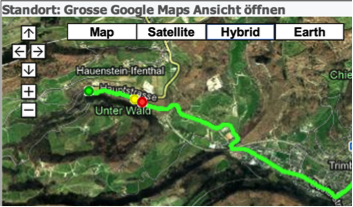
\includegraphics[width=100mm]{images/tourliveweb/kartenausschnitt.png}
	\caption{Die Positionen der Aufnahmegeräte}
\end{figure}
\subsection{Live Ticker}
Eine externe Person kann über ein Webinterface einen Live Ticker führen und Ereignisse während dem Rennen erfassen, diese werden dann sofort auf der Webseite dargestellt.
\subsection{Replay}
Das gesamte Rennen wird aufgezeichnet und kann später in Echtzeit oder im Schnelldurchlauf mit verschiedenen Geschwindigkeiten wiedergegeben werden. Je nach Rennen existieren mehrere Etappen, diese können dann einzeln ausgewählt werden. Die vergangenen Rennen können nach Jahr und Event sortiert und ausgewählt werden.
\subsection{Werbebanner}
Auf der Webseite wird ein Bereich definiert, in welchen Werbebanner dargestellt werden. Diese können in den Einstellungen ein und ausgeschaltet werden.
\subsection{Mobile Version}
Die Webseite soll auch auf Tablets und Smartphones sämtliche Informationen darstellen können. Dabei wird der Ansatz des Responsive Web Design verfolgt wobei die Clients die Webseite entsprechend ihrer Bildschirmgrösse rendern.
\begin{figure}[H]
	\centering 
	
\includegraphics[width=80mm]{images/tourliveweb/responsive.png}
	\caption{Die Darstellung der Webseite auf die Anzeigegrösse angepasst\footnote{Bildquelle:\url{http://johnpolacek.github.com/scrolldeck.js/decks/responsive/img/responsive_web_design.png}, Aufgerufen am 08.05.2013}}
\end{figure}
\subsection{Rennstandort (Marschtabelle)}
Die Besucher der TourLive Webseite können aufgrund Ihres aktuellen Standortes bestimmen, wann die Spitze am jeweiligen Ort eintreffen wird. Der Standort wird durch die Browser Geolocation API ermittelt damit kann dann die Distanz zur Spitze berechnet werden und aufgrund der Durchschnittsgeschwindigkeit den ungefähren Ankunftszeitpunkt.
Die ungefähren Ankunftszeiten gehen auch aus der Marschtabelle hervor. Diese lässt sich ebenfalls anzeigen.

\subsection{Abstandsentwicklung}
Die verschiedenen Aufnahmesysteme können sich unter Umständen weit voneinander entfernen. Die Entwicklung dieses Abstandes während des Rennen bietet für die Radsport-Kenner ein gutes Bild, wie sich das Feld verändert.
\begin{figure}[H]
	\centering
	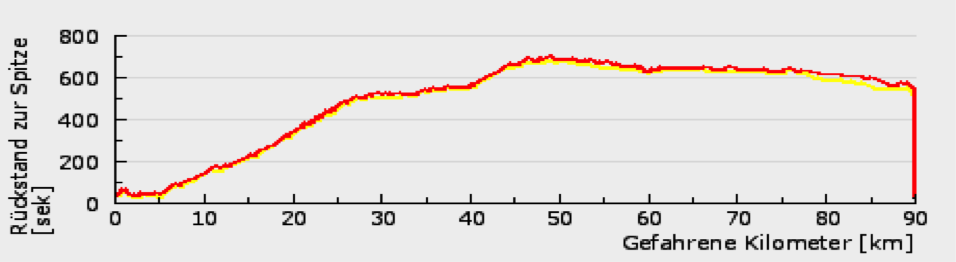
\includegraphics[width=100mm]{images/tourliveweb/abstandsentwicklung.png}
	\caption{Abstandsentwicklung nach Rennkilometer in Sekunden}
\end{figure}

\subsection{Public API}
Sämtliche Grafiken und Daten, welche auf der Webseite angezeigt werden, können auch einzeln über eine festgelegte Schnittstelle als JSON empfangen werden. Dies ermöglicht die Entwicklung von beliebigen Anwendungen durch Dritte. Den Zugang zur öffentlichen Schnittstelle wird durch einen API Key ermöglicht, einen solchen Key erhält, wer sich als Entwickler bei TourLive registriert; dadurch kann die Nutzung überwacht und allenfalls eingeschränkt werden.
\subsection{Input API}
Die aktuelle Rennsituation sowie weitere Informationen zum Rennen werden durch mehrere Android Geräte erfasst. Die Aufnahmegeräte senden sämtliche Informationen via JSON an die Serverschnittstelle. 
\\
Weiter werden Daten direkt vom RadioTour Speaker empfangen, diese liefern vor allem Informationen zur Situation im Rennfeld, wie viele Fahrer in welcher Formation fahren.
\subsection{Nutzungsstatisktik}
Über die Nutzung von TourLive wird eine Statistik geführt. Dabei wird auf eine bestehendes Web Analytics System zurückgegriffen, dieses System ist nicht Bestandteil der Arbeit es wird dabei auf Piwik oder Google verwendet.